% ============================================================
%  main.tex  —  WAND 7T fMRI Analysis
%  Compile with: pdflatex main.tex  (twice for references)
%                bibtex main        (if using references)
%                pdflatex main.tex
% ============================================================

\documentclass[11pt, a4paper]{article}

% ── Packages ─────────────────────────────────────────────────
\usepackage{fontspec}
\usepackage{microtype}

% Page geometry
\usepackage[
    top=2.5cm, bottom=2.5cm,
    left=2.5cm, right=2.5cm
]{geometry}

% Mathematics
\usepackage{amsmath, amssymb}

% Colours & graphics
\usepackage[dvipsnames,svgnames,x11names]{xcolor}

% Figures & tables
\usepackage{graphicx}
\usepackage{booktabs}
\usepackage{caption}
\usepackage{subcaption}
\usepackage{float}

% Hyperlinks (load last among most packages)
\usepackage[
    colorlinks=true,
    linkcolor=blue!70!black,
    citecolor=blue!70!black,
    urlcolor=blue!70!black
]{hyperref}

% Bibliography
\usepackage[numbers,sort&compress]{natbib}

% Line spacing
\usepackage{setspace}
\setstretch{1.2}

% Header / footer
\usepackage{fancyhdr}
\pagestyle{fancy}
\fancyhf{}
\rhead{\small WAND 7T fMRI Analysis}
\lhead{\small Kodwani \textit{et al.}}
\cfoot{\thepage}
\renewcommand{\headrulewidth}{0.4pt}

% ── Title ────────────────────────────────────────────────────
\title{
    \textbf{Resting-State fMRI Data Quality and Analysis\\
    in the WAND 7T Dataset}\\[0.5em]
    \large A Comparative Evaluation of Preprocessing Pipelines
}

\author{
    Darsh Kodwani\\
    \small Cardiff University Brain Research Imaging Centre (CUBRIC)\\
    \small \texttt{d.kodwani@cardiff.ac.uk}
}

\date{March 2026}

% ============================================================
\begin{document}
% ============================================================

\maketitle
\thispagestyle{fancy}
\tableofcontents
\newpage

% ─────────────────────────────────────────────────────────────
\begin{abstract}
% ─────────────────────────────────────────────────────────────

% TODO: Write abstract (~200 words)
%
% Suggested content:
%   - Brief description of the WAND dataset (7T, resting-state, N subjects)
%   - Motivation: understanding data quality before functional analysis
%   - Key approach: comparative evaluation of preprocessing steps
%     (motion correction, brain masking) against MRIQC reference values
%   - Main finding: ~61% improvement in tSNR with motion correction;
%     mask choice (nilearn EPI mask) explains an additional ~10%
%   - Conclusion: dataset is suitable for group-level connectivity analyses
%     with recommended preprocessing pipeline

\noindent
\textit{Placeholder --- write abstract here.}

\end{abstract}

\newpage

% ─────────────────────────────────────────────────────────────
\section{Introduction \& Context}
\label{sec:intro}
% ─────────────────────────────────────────────────────────────

% TODO: Introduce the WAND dataset and scientific context.
%
% Suggested structure:
%   1. Background on 7T fMRI — advantages (spatial resolution, SNR)
%      and challenges (B1 inhomogeneity, physiological noise, SAR)
%   2. Description of the WAND dataset:
%      - N subjects, sessions, acquisition parameters (1.5 mm isotropic,
%        TR = 1.5 s, multiband acceleration)
%   3. Motivation for a systematic QC evaluation before analysis
%   4. Overview of MRIQC as a reference standard
%   5. Aims of this paper

\subsection{7T fMRI: Opportunities and Challenges}

\subsection{The WAND Dataset}

\subsection{Aims}

% ─────────────────────────────────────────────────────────────
\section{Pre-processing and Data Quality}
\label{sec:preprocessing}
% ─────────────────────────────────────────────────────────────

% TODO: Describe the preprocessing pipeline and QC metrics.
%
% Suggested structure:
%   1. Image quality metrics (IQMs) — tSNR, CoV, DVARS, GCOR
%   2. Baseline pipeline (raw): simple intensity mask, no motion correction
%   3. Motion correction: FSL mcflirt, reference volume, dummy TR removal
%   4. Brain masking: simple intensity threshold vs nilearn compute_epi_mask
%   5. Group-level QC: histogram of tSNR across all N subjects
%   6. Comparison with MRIQC reference values

\subsection{Image Quality Metrics}

The temporal signal-to-noise ratio (tSNR) is defined voxel-wise as:

\begin{equation}
    \text{tSNR}(\mathbf{x}) = \frac{\bar{S}(\mathbf{x})}{\sigma_t(\mathbf{x})}
    \label{eq:tsnr}
\end{equation}

where $\bar{S}(\mathbf{x})$ is the temporal mean and $\sigma_t(\mathbf{x})$ is
the temporal standard deviation of the BOLD signal at voxel $\mathbf{x}$.
The group-level metric reported is the median tSNR across all brain voxels.

\subsection{Motion Correction}

\subsection{Brain Masking}

\subsection{Group-Level Quality Assessment}

% Example figure placeholder:
% \begin{figure}[H]
%     \centering
%     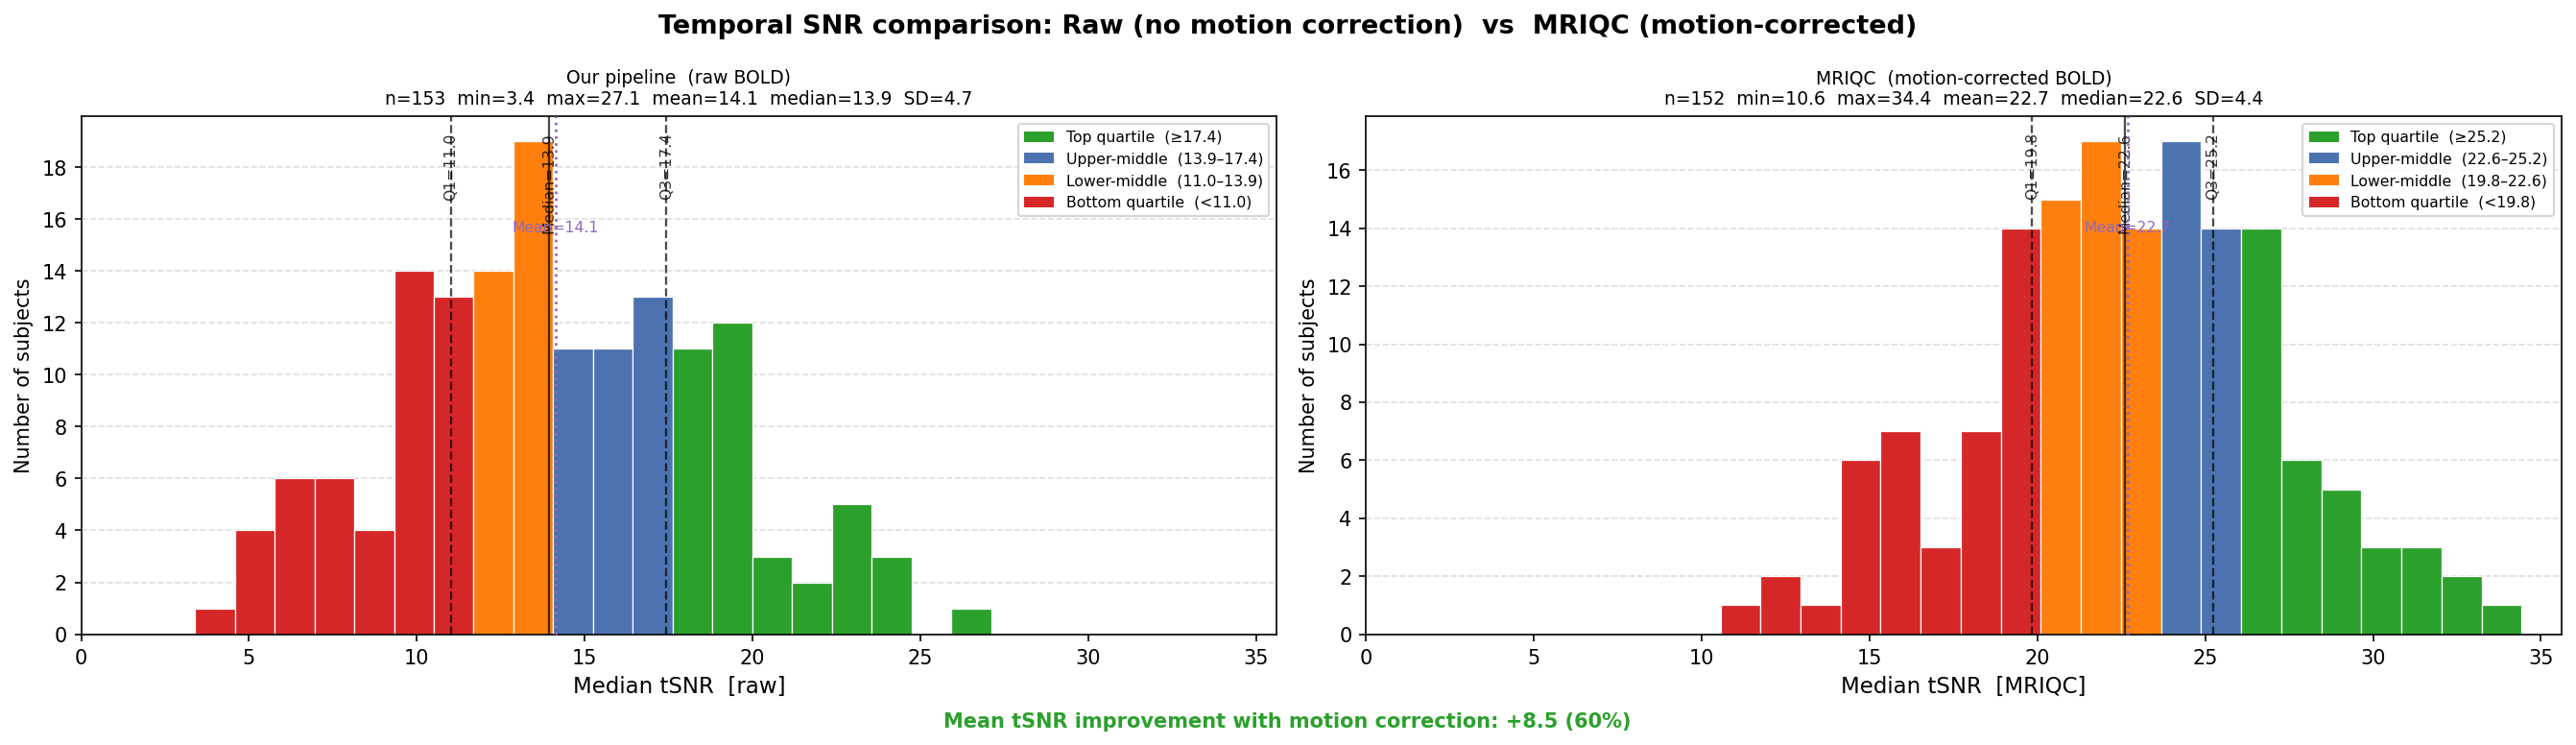
\includegraphics[width=0.8\textwidth]{../../results/group/tsnr_comparison.png}
%     \caption{Comparison of median tSNR distributions across all subjects
%              before (left) and after (right) motion correction and improved
%              brain masking. Colours indicate quartile membership.}
%     \label{fig:tsnr_comparison}
% \end{figure}

\subsection{Preprocessing Pipeline Comparison}

% Example table:
\begin{table}[H]
    \centering
    \caption{tSNR for subject sub-01187 under four preprocessing conditions.
             MRIQC value serves as the reference standard.}
    \label{tab:preprocessing_comparison}
    \begin{tabular}{lrr}
        \toprule
        \textbf{Condition} & \textbf{tSNR} & \textbf{$\Delta$ vs MRIQC} \\
        \midrule
        Raw + simple intensity mask (baseline) & 21.18 & $-7.43$ ($-26.0\%$) \\
        Raw + nilearn EPI mask                 & 25.78 & $-2.83$ ($-9.9\%$)  \\
        Moco + simple intensity mask           & 26.85 & $-1.77$ ($-6.2\%$)  \\
        Moco + nilearn EPI mask                & 31.45 & $+2.83$ ($+9.9\%$)  \\
        \midrule
        MRIQC reference                        & 28.62 & ---                  \\
        \bottomrule
    \end{tabular}
\end{table}

% ─────────────────────────────────────────────────────────────
\section{Analysis Methods}
\label{sec:methods}
% ─────────────────────────────────────────────────────────────

% TODO: Describe the functional analysis methods.
%
% Suggested structure:
%   1. Software environment (Python, FSL, nilearn versions)
%   2. Subject selection criteria based on QC thresholds
%   3. fMRI preprocessing pipeline (full, including moco) for analysis
%   4. Connectivity / GLM analysis approach
%   5. Statistical inference

\subsection{Software and Environment}

\subsection{Subject Selection}

\subsection{fMRI Preprocessing}

\subsection{Functional Connectivity Analysis}

\subsection{Statistical Analysis}

% ─────────────────────────────────────────────────────────────
\section{Results}
\label{sec:results}
% ─────────────────────────────────────────────────────────────

% TODO: Present results.
%
% Suggested structure:
%   1. Data quality summary across cohort (tSNR, DVARS, motion)
%   2. Subject exclusions based on QC criteria
%   3. Main functional analysis results

\subsection{Data Quality Across the Cohort}

\subsection{Subject Exclusions}

\subsection{Functional Analysis Results}

% ─────────────────────────────────────────────────────────────
\section{Summary}
\label{sec:summary}
% ─────────────────────────────────────────────────────────────

% TODO: Summarise findings and discuss implications.
%
% Suggested structure:
%   1. Key finding: preprocessing choice substantially affects tSNR
%   2. Interpretation of cohort-level data quality
%   3. Limitations (e.g. no NORDIC, no physiological denoising)
%   4. Future directions

\subsection{Key Findings}

\subsection{Limitations}

\subsection{Future Directions}

% ─────────────────────────────────────────────────────────────
% References
% ─────────────────────────────────────────────────────────────
\newpage
\bibliographystyle{unsrtnat}
\bibliography{references}

% ============================================================
\end{document}
% ============================================================
